%
% This is a borrowed LaTeX template file for lecture notes for CS267,
% Applications of Parallel Computing, UCBerkeley EECS Department.
%

\documentclass{article}
\usepackage{titlesec}
%\setlength{\oddsidemargin}{0.25 in}
%\setlength{\evensidemargin}{-0.25 in}
\setlength{\oddsidemargin}{0 in}
\setlength{\evensidemargin}{0 in}
\setlength{\topmargin}{-0.6 in}
\setlength{\textwidth}{6.5 in}
\setlength{\textheight}{8.5 in}
\setlength{\headsep}{0.75 in}
\setlength{\parindent}{0 in}
\setlength{\parskip}{0.1 in}


%
% ADD PACKAGES here:
%

\usepackage{amssymb}	% Already loads amsfonts
\usepackage{amsthm}
\usepackage{graphicx}
\usepackage{mathtools}	% Already loads amsmath
\usepackage{hyperref}
\usepackage{enumitem}
\usepackage{clrscode3e}  % for typesetting pseudocode
\usepackage{ulem}
\usepackage[usenames,dvipsnames]{xcolor}
\usepackage{multicol}


% Tikz and setup
\usepackage{tikz}
\usepackage{tikz-cd}
\usetikzlibrary{intersections, angles, quotes, calc, positioning}
\usetikzlibrary{arrows.meta}
\usepackage{pgfplots}
\pgfplotsset{compat=1.13}


\tikzset{
    force/.style={thick, {Circle[length=2pt]}-stealth, shorten <=-1pt}
}

%
% The following commands set up the lecnum (lecture number)
% counter and make various numbering schemes work relative
% to the lecture number.
%
\newcounter{lecnum}
\renewcommand{\thepage}{\thelecnum-\arabic{page}}
\renewcommand{\thesection}{\thelecnum.\arabic{section}}
\renewcommand{\theequation}{\thelecnum.\arabic{equation}}
\renewcommand{\thefigure}{\thelecnum.\arabic{figure}}
\renewcommand{\thetable}{\thelecnum.\arabic{table}}

%
% The following macro is used to generate the header.
%
\newcommand{\lecture}[5]{
   \pagestyle{myheadings}
   \thispagestyle{plain}
   \newpage
   \setcounter{lecnum}{#2}
   \setcounter{page}{1}
   \noindent
   \begin{center}
   \framebox{
      \vbox{\vspace{2mm}
    \hbox to 6.28in { {\bf #1
	\hfill} }
       \vspace{4mm}
       \hbox to 6.28in { {\Large \hfill Lecture #2: #3  \hfill} }
       \vspace{2mm}
       \hbox to 6.28in { {\it Lecturer: #4 \hfill Scribe: #5} }
      \vspace{2mm}}
   }
   \end{center}
   \markboth{Lecture #2: #3}{Lecture #2: #3}
   \vspace*{4mm}
}
\renewcommand{\cite}[1]{[#1]}
\def\beginrefs{\begin{list}%
        {[\arabic{equation}]}{\usecounter{equation}
         \setlength{\leftmargin}{2.0truecm}\setlength{\labelsep}{0.4truecm}%
         \setlength{\labelwidth}{1.6truecm}}}
\def\endrefs{\end{list}}
\def\bibentry#1{\item[\hbox{[#1]}]}

\newcommand{\fig}[3]{
			\vspace{#2}
			\begin{center}
			Figure \thelecnum.#1:~#3
			\end{center}
	}

% Colored theorem styles
\makeatother
\usepackage{thmtools}
\usepackage[framemethod=TikZ]{mdframed}
\mdfsetup{skipabove=1em,skipbelow=1em}

\declaretheoremstyle[
    headfont=\bfseries\sffamily\color{ForestGreen!70!black}, bodyfont=\normalfont,
    mdframed={
        linewidth=2pt,
        rightline=false, topline=false, bottomline=false,
        linecolor=ForestGreen, backgroundcolor=ForestGreen!5,
    },
    spaceabove=8pt
]{thmgreenbox}

\declaretheoremstyle[
    headfont=\bfseries\sffamily\color{NavyBlue!70!black}, bodyfont=\normalfont,
    mdframed={
        linewidth=2pt,
        rightline=false, topline=false, bottomline=false,
        linecolor=NavyBlue, backgroundcolor=NavyBlue!5,
    },
    spaceabove=8pt
]{thmbluebox}

\declaretheoremstyle[
    headfont=\bfseries\sffamily\color{NavyBlue!70!black}, bodyfont=\normalfont,
    mdframed={
        linewidth=2pt,
        rightline=false, topline=false, bottomline=false,
        linecolor=NavyBlue
    },
    spaceabove=8pt
]{thmblueline}

\declaretheoremstyle[
    headfont=\bfseries\sffamily\color{RawSienna!70!black}, bodyfont=\normalfont,
    mdframed={
        linewidth=2pt,
        rightline=false, topline=false, bottomline=false,
        linecolor=RawSienna, backgroundcolor=RawSienna!5,
    },
    spaceabove=8pt
]{thmredbox}

\declaretheoremstyle[
    headfont=\bfseries\sffamily\color{RawSienna!70!black}, bodyfont=\normalfont,
    numbered=no,
    mdframed={
        linewidth=2pt,
        rightline=false, topline=false, bottomline=false,
        linecolor=RawSienna, backgroundcolor=RawSienna!1,
    },
    qed=\qedsymbol,
    spaceabove=8pt
]{thmproofbox}

\declaretheoremstyle[
    headfont=\bfseries\sffamily\color{NavyBlue!70!black}, bodyfont=\normalfont,
    numbered=no,
    mdframed={
        linewidth=2pt,
        rightline=false, topline=false, bottomline=false,
        linecolor=NavyBlue, backgroundcolor=NavyBlue!1,
    },
    spaceabove=8pt
]{thmexplanationbox}

% Use these for theorems, lemmas, proofs, etc.
\theoremstyle{definition}
\declaretheorem[style=thmgreenbox, name=Definition, numberwithin=lecnum]{definition}
\declaretheorem[style=thmbluebox, numbered=no, name=Example]{example}
\declaretheorem[style=thmredbox, name=Theorem, numberwithin=lecnum]{theorem}
\declaretheorem[style=thmredbox, name=Proposition, sibling=theorem]{proposition}
\declaretheorem[style=thmredbox, name=Lemma, sibling=theorem]{lemma}
\declaretheorem[style=thmredbox, name=Corollary, sibling=theorem]{corollary}
% \newtheorem{theorem}{Theorem}[lecnum]
% \newtheorem{lemma}[theorem]{Lemma}
% \newtheorem{claim}[theorem]{Claim}
% \newtheorem{corollary}[theorem]{Corollary}
% \newtheorem{definition}[theorem]{Definition}
\declaretheorem[style=thmblueline, numbered=no, name=Remark]{remark}
\renewenvironment{proof}{{\bf \textit{Proof.}}}{\hfill\rule{2mm}{2mm}}
\makeatletter


% **** IF YOU WANT TO DEFINE ADDITIONAL MACROS FOR YOURSELF, PUT THEM HERE:

\renewcommand\Pr{\mathbb{P}}
\newcommand\Ex{\mathbb{E}}

\newcommand\N{\mathbb{N}}
\newcommand\Z{\mathbb{Z}}
\newcommand\Q{\mathbb{Q}}
\newcommand\R{\mathbb{R}}
\newcommand\C{\mathbb{C}}
\newcommand\F{\mathbb{F}}

\DeclarePairedDelimiter\ceil{\lceil}{\rceil}
\DeclarePairedDelimiter\floor{\lfloor}{\rfloor}
\DeclarePairedDelimiter\anglebrac{\langle}{\rangle}

\begin{document}
\lecture{MAT344 Intro to Combinatorics}{7}{Intro to Graph Theory}{Keegan Dasilva Barbosa}{Kevin Gao}

\section{Graphs}

We begin by providing a formal definition of graphs.

\begin{definition}[Undirected Graph]
    A (undirected) \textit{\textbf{graph}} is a pair $(V,E)$ where $V$ is a finite set, and $E$ is a collection of subsets of $V$ of size 2. The set $V$ is called the vertex set, and members of $V$ are called \textbf{vertices}. The set $E$ is called the edge set and members of $E$ are called \textbf{edges}.
\end{definition}

We generally use $G$ to denote a graph. For $x,y \in V$, the edge between $x$ and $y$ is denoted $\{x,y\}$, or sometimes $xy$ or $yx$. The set notation $\{\cdot\}$ is to highlight the unordered nature of an undirected edge. If $x, y \in V$ and $\{x,y\} \in E$, we say that $x$ and $y$ are \textbf{adjacent}.

\section{Classic Graphs}

\begin{definition}[Complete Graph]
    For $n \geq 1$, we let $K_n$ denote the complete graph $([n], E)$ where $E = \{e \subseteq [n] \mid |e| = 2\}$.
\end{definition}

Conversely, if for all distinct $x,y \in V$, $\{x,y\} \not\in E$, the graph is called an independent graph, denoted $I_n$.

\begin{definition}[Path Graph]
    For $n \geq 1$, we let $P_n$ denote the path graph $([n], E)$ where $E = \{ \{i,i+1\} \subseteq [n] \mid i \in [n] \}$.
\end{definition}

\begin{definition}[Cycle Graph]
    For $n \geq 3$, we let $C_n$ denote the cycle graph $([n], E)$ where $E = \{ \{0,1\},\, \{1,2\},\, \ldots,\, \{n-2,n-1\},\, \{n-1,0\} \}$.
\end{definition}

\begin{figure}[htbp]
    \centering
    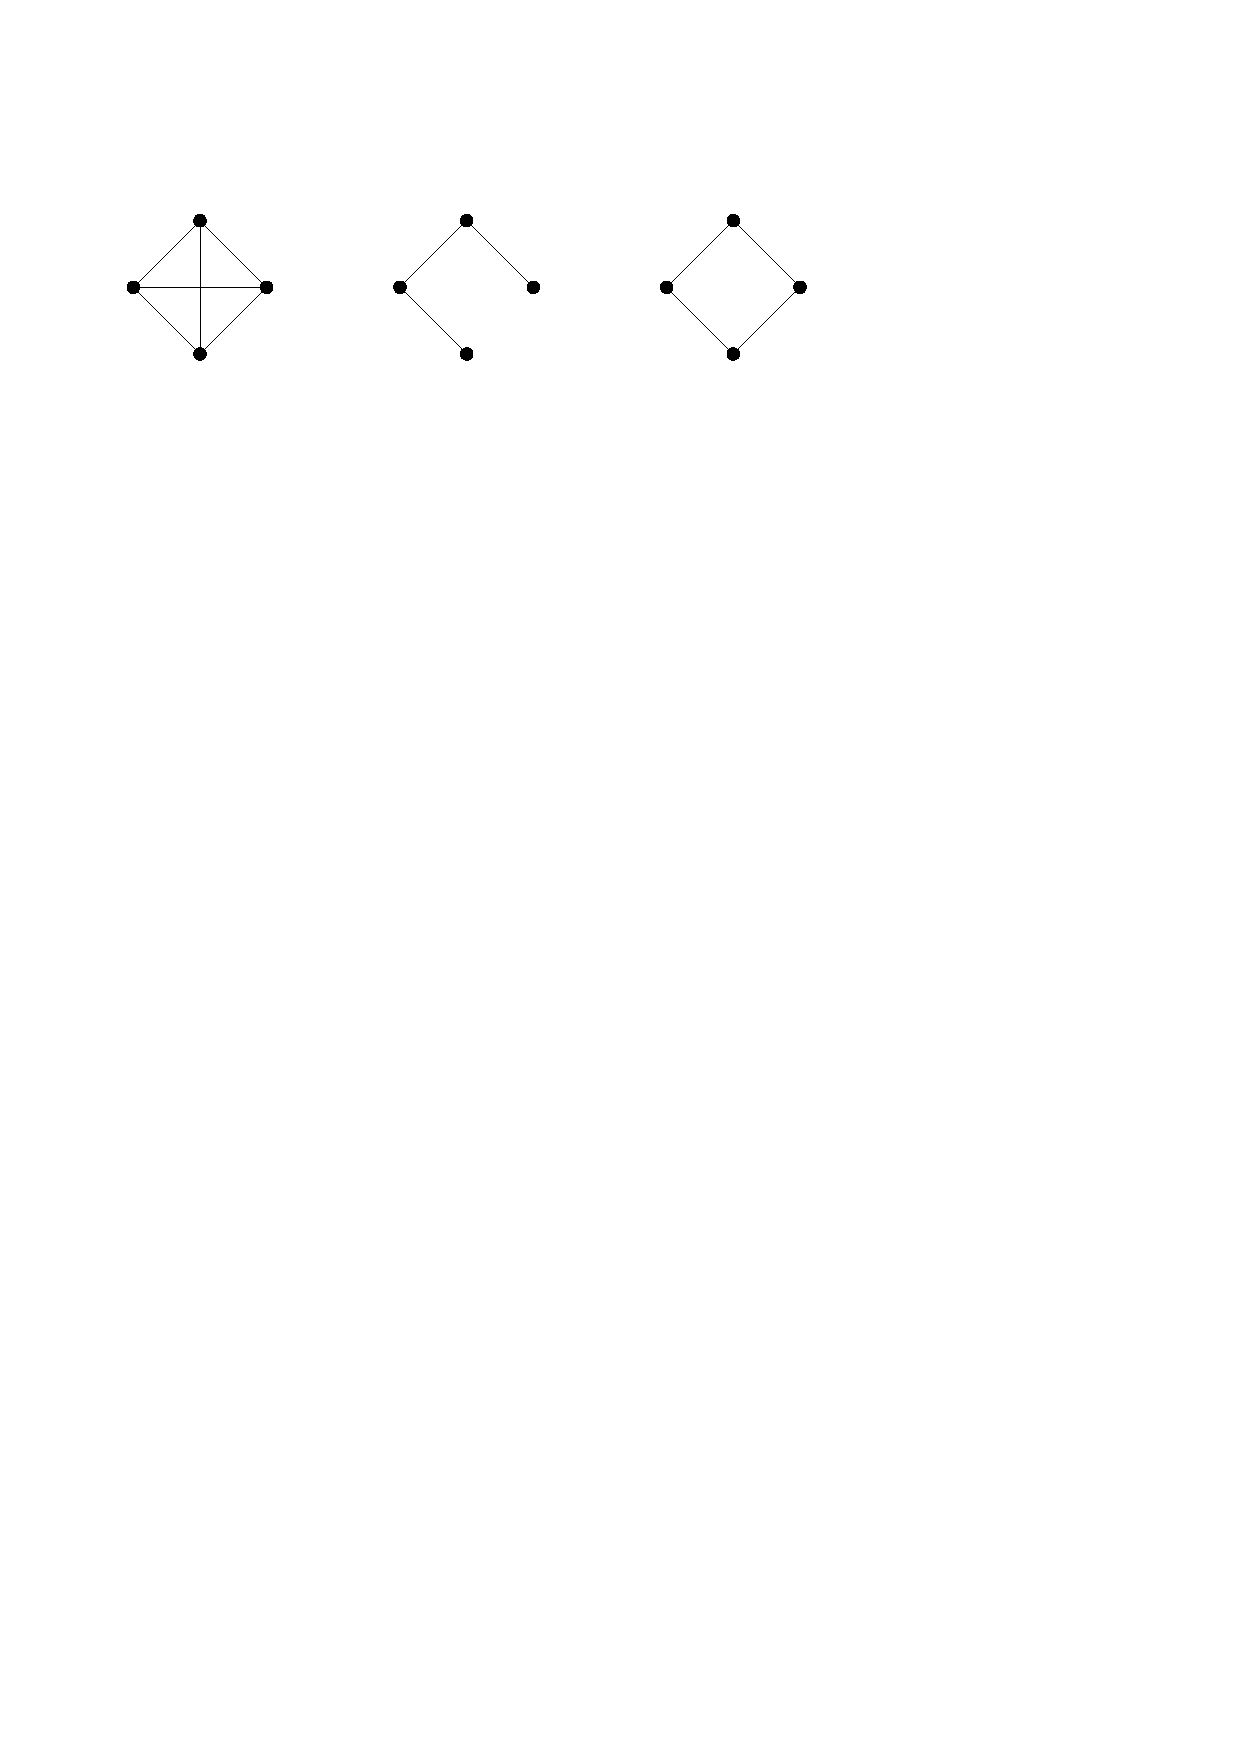
\includegraphics[width=0.6\linewidth]{figures/classic-graphs.pdf}
    \caption{From left to right: complete graph, path graph, cycle graph with 4 vertices.}
    \label{fig:classic-graphs}
\end{figure}

\section{Subgraphs}

\subsection{Definitions}

\begin{definition}[Subgraph]
    Given a graph $G = (V,E)$, a \textit{\textbf{subgraph}} $H$ of $G$ is a pair $H = (W,E')$ such that $W \subseteq V$ and $E' \subseteq \{s \in E \mid s \subseteq W\}$.
\end{definition}

Sometimes, we abuse notation and write $H \subseteq G$.

\begin{definition}[Induced Subgraph]
    Given a graph $G = (V,E)$, an \textit{\textbf{induced subgraph}} $H \subseteq G$ is one of the form $(W,E')$ where
    $$
    E' = \{ \{x,y\} \in E \mid \{x,y\} \in W\}
    $$
    for $W \subseteq V$.
\end{definition}

Note that induced subgraphs are uniquely defined by the vertex set whereas a subgraph is not. A subgraph need not contain all edges between the vertices in the subgraph.

\subsection{Isomorphism}

\begin{definition}[Isomorphic Graphs]
    Let $G = (V_1,E_1)$ and $H = (V_2,E_2)$ be graphs. We say that $G$ and $H$ are isomorphic if there is a bijection $f:\; V_1 \to V_2$ such that $\{x,y\} \in E_1 \iff \{f(x),f(y)\} \in E_2$.
\end{definition}

\begin{theorem}
    Let $G$ be a graph with $n$ vertices. $G$ is isomorphic to a subgraph of $K_n$.
\end{theorem}

\begin{proof}
    Consider $G = (V,E)$. Label the vertices such that $V = \{v_0,\ldots,v_{n-1}\}$. Let $f:\; V \to [n]$ be a function such that $f(v_i) = i$. Consider the set $E' = \{\{i,j\} \subseteq [n] \mid \{v_i,v_j\} \in E\}$. Clearly, $H = ([n], E')$ is a subgraph of $K_n$ by definition. Further, we claim that $f$ is an isomorphism between $G$ and $H$.
    
    To show that $f$ is an isomorphism, it suffices to show that $\{v_i,v_j\} \in E \iff \{f(i),f(j)\} \in E'$. For the forward direction, suppose $\{v_i,v_j\} \in E$, then $\{i,j\} \in E'$ by construction. This immediately implies that $\{f(v_i),f(v_j)\} \in E'$ by construction of $f$. For the reverse direction, suppose $\{i,j\} \in E'$, which is equivalent to $\{f(v_i),f(v_j)\} \in E'$. By definition of $f$, this is only true when $\{v_i,v_j\} \in E$. Therefore, $f$ is an isomorphism between $G$ and $H$.
    
    It follows that $G$ is isomorphic to $H$, which is a subgraph of $K_n$.
\end{proof}

\section{Degrees and Degree Sequence}

\begin{definition}[Degree]
    Given a graph $G = (V,E)$ and a vertex $v \in V$, we let $\deg_G(v) = |\{u \in V \mid \{u,v\} \in E\}|$, which is the number of vertices ahring an edge with $v$.
\end{definition}

\begin{definition}[Degree Sequence]
    Given a graph $G$, we can create a sequence $(\deg_G(v) \mid v \in V)$ of degrees called a degree sequence.
\end{definition}

\begin{theorem}
    Let $G = (V_1,E_1)$ and $H = (V_2,E_2)$ be graphs, and let $f:\; G \to H$ be an isomorphism. Then, $\deg_G(v) = \deg_H(f(v))$.
\end{theorem}

\begin{proof}
    Let $f:\; G \to H$ be an isomorphism. For each $v \in V_1$, consider the sets
    $$
    \{w \in V_1 \mid \{v,w\} \in E_1\}
    $$
    and
    $$
    \{y \in V_2 \mid \{f(v),y\} \in E_2\}.
    $$
    Since $f$ is an isomorphism, each $v \in V_1$ is mapped to one and only one vertex in $V_2$. Further, $\{v,w\} \in E_1 \iff \{f(v),f(w)\} \in E_2$. Then, the two sets have the same cardinality. By definition, this means $\deg_G(v) = \deg_H(f(v))$ for all $v \in V_1$.
\end{proof}

This theorem provides us with a quick way to check if two graphs are isomorphic. We can check this by simply checking the degree and/or degree sequence instead of considering the actual isomorphism mapping.

\begin{corollary}
    If $G$ and $H$ have different degree sequences (under a given ordering of the sequence), then they are not isomorphic.
\end{corollary}

\begin{lemma}[The Handshaking Lemma]
    Let $G=(V,E)$ be a graph, and let $|E| = e$. Then,
    $$
    \sum_{v \in V} \deg_G(v) = 2e
    $$
\end{lemma}

\begin{proof}
    For each $v \in V$, let $E_V = \{\{v,u\} \mid \{v,u\} \in E\}$. Notice that for distinct $u,v$, $|E_u \cap E_v| \leq 1$ and is equal to one exactly when $u$ and $v$ form an edge. No three distinct sets overlap. It follows that
    $$
    e = |E| = \left| \bigcup_{v \in V} E_v \right| = \sum_{v \in V} |E_v| - \sum_{u,v \in V} |E_v \cap E_u| = \sum_{v \in V} \deg_G(v) - e
    $$
    This implies $\sum_{v \in V} \deg_G(v) = 2e$.
\end{proof}

\section{Connectivity}

\begin{definition}[Path]
    A \textit{\textbf{path}} in a graph $G = (V,E)$ is a sequence of \textbf{distinct} vertices $x_1,\ldots,x_n$ that are each successively connected with an edge. We call the number of edges in the sequence the length of the path.
\end{definition}

\begin{definition}[Walk]
    A \textit{\textbf{walk}} in a graph $G = (V,E)$ is a sequence of vertices that are each successively connected with an edge.
\end{definition}

Note that a walk does not have the distinctness requirement, meaning repeating vertices in a walk is allowed.

\begin{definition}[Connectivity]
    We call a graph $G$ connected if every pair of distinct vertices is connected by a path.
\end{definition}

\begin{definition}[Connected Component]
    Given a graph $G$, we call a maximally connected vertex set a \textit{\textbf{connected component}}. More formally, if we denote the equivalence relation $\sim$ on $V$ given by
    $$
    v \sim w \iff v = w
    $$
    (i.e. $v$ is connected to $w$), the \textit{\textbf{connected components}} are the equivalence classes given by this relation.
\end{definition}

\section{Trees and Spanning Trees}

\subsection{Definition and a Useful Theorem}

\begin{definition}[Tree]
    A \textit{\textbf{tree}} is a graph $G = (V,E)$ with the property that every two vertices are connected by a \textbf{unique} path.
\end{definition}

\begin{lemma} \label{lem:acyclic-graph-degree}
    Every acyclic and connected graph $G$ with $n \geq 2$ vertices has a leaf $v \in V$ such that $\deg(v) = 1$.
\end{lemma}

\begin{proof}
    Let $G$ be an acyclic and connected graph. Note that since $G$ is connected, $\deg_G(v) \geq 1$ for all $v \in V$. We prove the contrapositive. Suppose for all $v \in V$, $\deg_G(v) > 1$. Fix a vertex $v$. Starting from $v$, follow a sequence of distinct edges until a vertex repeats. It is possible to visit all vertices without repeating edges because each vertex has two incident edges. Further, because every vertex has degree of at least 2, once we have visited every vertex, there should still be at least one edge unvisited. When we follow that edge, we will arrive at a vertex that has previously been visited. This creates a cycle. So, $G$ is not acyclic.
\end{proof}

\begin{theorem} \label{thm:equiv-tree-def}
    Let $G$ be a \textbf{connected graph} with $n$ edges. The following are equivalent:
    \begin{enumerate}
        \item $G$ is a tree
        \item $G$ does not contain a cycle
        \item $G$ has $n-1$ edges
    \end{enumerate}
\end{theorem}

\begin{proof}
    Let $G$ be a connected graph.

    (1 $\implies$ 2): Assume that $G$ is a tree. We show that $G$ does not contain a cycle by contradiction, so suppose not and $G$ contains a cycle. Let the cycle be $c = x_1x_2\ldots x_n$. Notice that $x_1x_2\ldots x_n$ is a path from $x_1$ to $x_n$. Since $c$ is a cycle, $\{x_1,x_n\} \in E$. So, $x_1x_n$ is also a path from $x_1$ to $x_n$. However, this is a contradiction to the path uniqueness requirement in the definition of a tree. So $G$ does not contain a cycle.

    (2 $\implies$ 3): We prove this implication by induction. Assume $G$ is acyclic and connected.

    \textbf{Base Case}: $n = 1$. There is $0 = n-1$ edge. The implication holds.

    \textbf{Inductive Step}: Let $n \in \N$ and $n \geq 2$. As induction hypothesis, suppose all acyclic and connected graphs with $m \leq n$ vertices have $m-1$ edges. Let $G$ be a graph with $n+1$ vertices. Suppose that $G$ is also connected and acyclic. By Lemma \ref{lem:acyclic-graph-degree}, $G$ has at least one vertex $v$ such that $\deg_G(v) = 1$. Construct $G'$ by removing $v$ and the one edge incident to $v$. $G'$ has $n$ vertices, so by induction hypothesis, has $n-1$ edges. If we add back the removed edge, we can see that $G$ has $n$ edges.

    By induction, this implication holds.

    (3 $\implies$ 1): Let $G$ be a connected graph with $n-1$ edges. To show that $G$ is a tree, we need to show that every two vertices are connected by a unique path. It suffices to show that deleting any edge from $G$ leaves the graph disconnected. Suppose for contradiction that deleting an edge $\{u,v\}$ does not disconnect the graph. This implies that there is another path from $u$ to $v$ containing at least 2 edges. This also implies that $G$ is connected with $n-2$ edges. But this is impossible because the minimum number of edges in a connected graph with $n$ vertices is $n-1$. Therefore, every pair of vertices is connected via a unique path since deleting any edge breaks this path and thus disconnects the graph. By definition, this means $G$ is a tree.
\end{proof}

\begin{definition}
    Let $T = (V,E)$ be a tree. We call a vertex $v$ a leaf if $\deg_T(v) = 1$.
\end{definition}

\begin{lemma}
    If $G = (V,E)$ is a tree with $n \geq 2$ vertices, then $G$ has at least two leaves.
\end{lemma}

\begin{proof}
    We prove this lemma by strong induction on $n$ for $n \geq 2$.

    \textbf{Base Case}: $n = 2$. Since $T$ is a tree, $T$ is connected and has exactly one edge. Clearly, both vertices in $T$ have degree 1.

    \textbf{Inductive Step}: Suppose, as inductive hypothesis, that for some $n \geq 2$, every tree with $2 \leq k \leq n$ vertices has at least two leaves. Let $T$ be a tree with $n+1$ vertices. Pick an edge $\{u,v\} \in E$ and form a new graph $T'$ by deleting $\{u,v\}$. More formally, $T' = (V, E - \{\{u,v\}\})$. Since $T$ is a tree, there is no other path between $u$ and $v$ (otherwise we would have a cycle). It follows that in $T'$, $u$ and $v$ are disconnected. Deleting an edge will not create a cycle either, so $T'$ is a forest with two connected components $T_u$ and $T_v$. Consider the following cases:

    Case 1: Both $T_u$ and $T_v$ contain at least 2 vertices. Then, we can apply our induction hypothesis. Take one leaf from each component. If both are endpoints of the deleted edge $\{u,v\}$, they are no longer leaves in $T$, but we still have at least two leaves, one from $T_u$ and one from $T_v$. In general, $T_u$ must have a leaf $x$ that is not $u$ and $T_v$ must have a leaf $y$ that is not $v$. Adding $\{u,v\}$ back does not affect $x$ and $y$ so they will remain leaves, which implies that there exist at least two leaves.
    
    Case 2: If each component of $T'$ has only one vertex, then $T$ is isomorphic to $K_2$, which has two leaves.
    
    Case 3: If exactly one of the components has only one vertex, then it must become a leaf when we reconnect $\{u,v\}$ to form $T$.

    In all cases, we have that $T$ has at least two leaves. By induction, every tree with at least 2 vertices has at least two leaves.
\end{proof}

\begin{figure}[htbp]
    \centering
    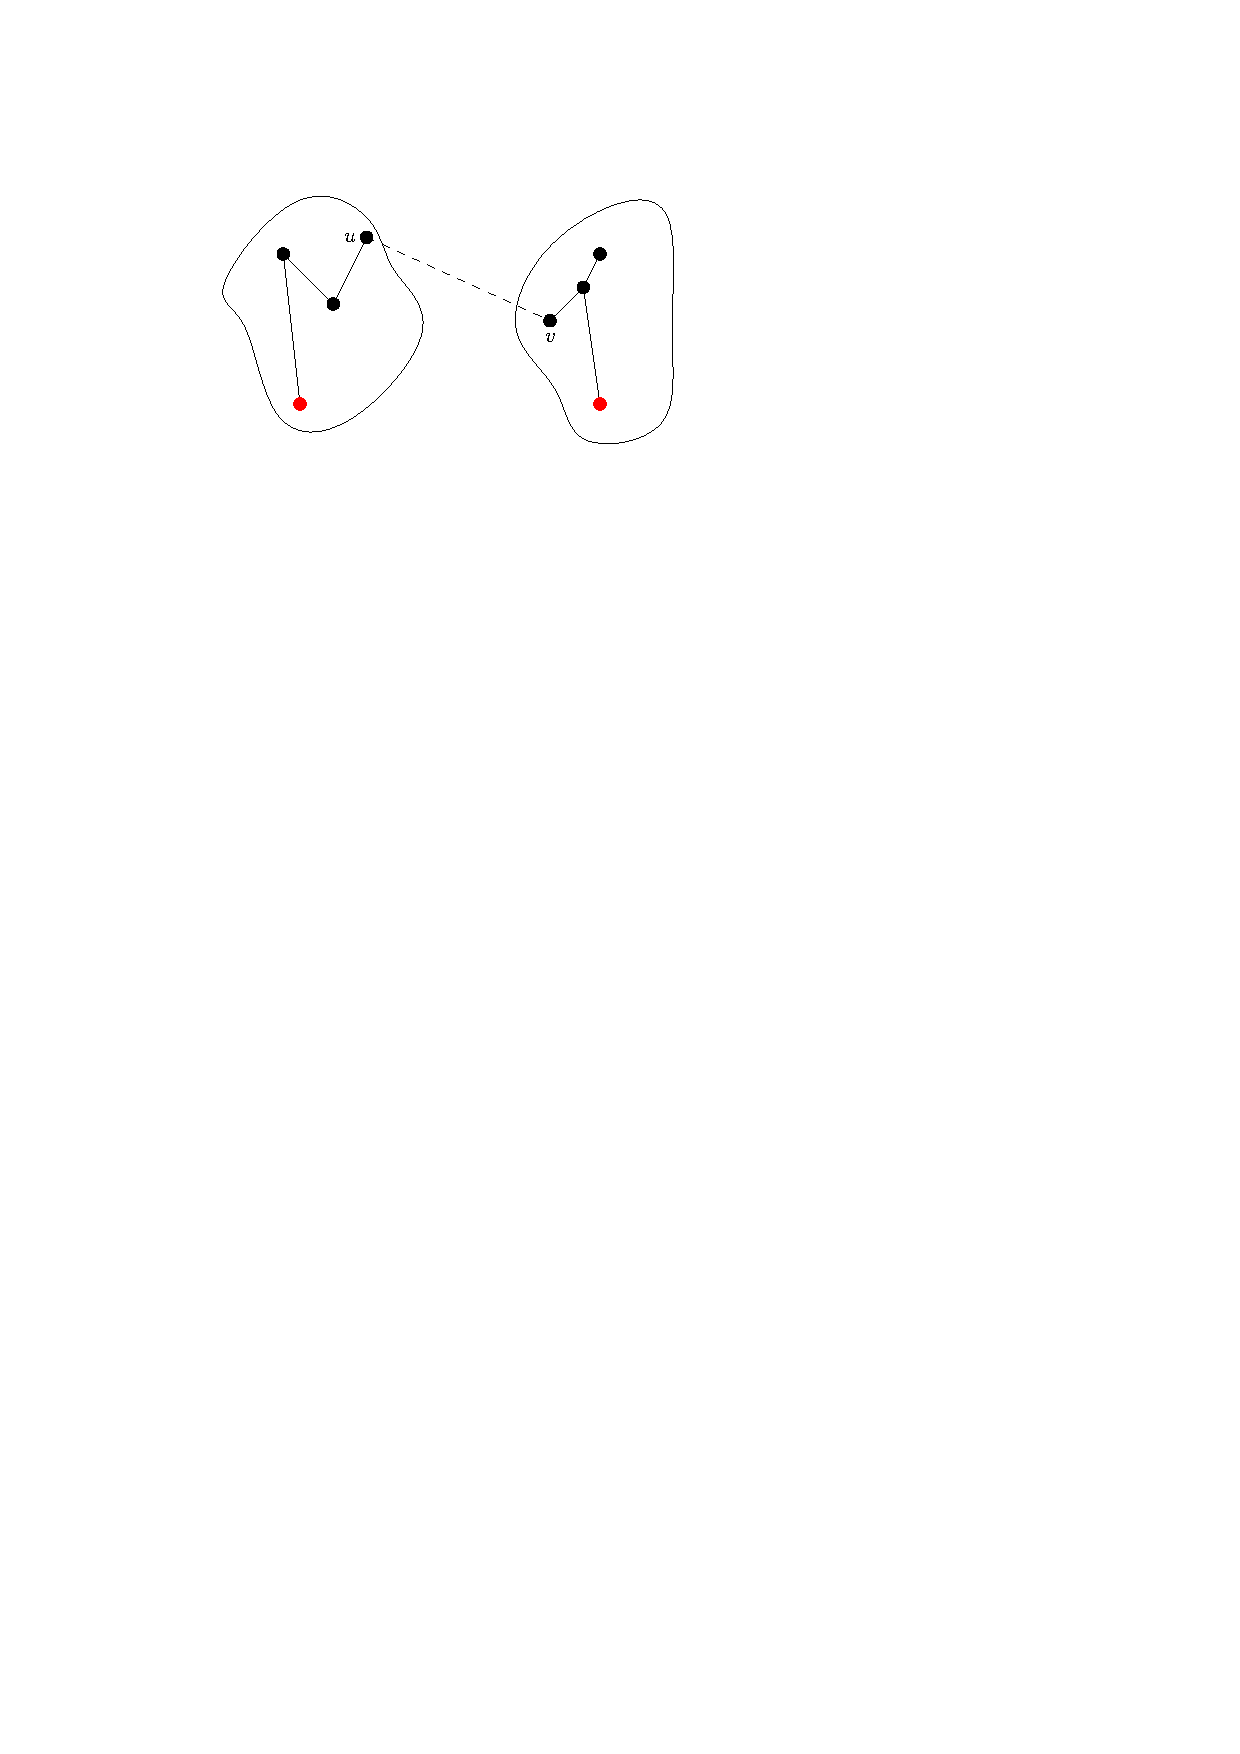
\includegraphics[width=0.4\linewidth]{figures/pendant-vertex-cycle.pdf}
    \caption{In each of the two components, there exists at least one leaf that is not $u$ or $v$ (colored red). When we reconnect $\{u,v\}$, those vertices will remain leaves.}
    \label{fig:pendant-vertex}
\end{figure}

\subsection{Spanning Trees}

\begin{definition}[Spanning Subgraph]
    Given a graph $G = (V,E)$, we call a subgraph $H \subseteq G$ \textit{\textbf{spanning}} if $H = (V,E')$.
\end{definition}

\begin{definition}[Spanning Tree]
    Given a graph $G$, a \textit{\textbf{spanning tree}} is a spanning subgraph $T \subseteq G$ that is a tree.
\end{definition}

\begin{theorem}
    Every connected graph has a spanning tree.
\end{theorem}

\begin{proof}
    By induction on the number of edges.

    \textbf{Base Case}: If $G$ is connected and has no edges, $G$ contains one single vertex. $G$ is trivially a tree and a spanning tree.

    \textbf{Inductive Step}: Suppose $G$ has $m \geq 1$ edges. If $G$ is a tree, then we are done because it is trivially a spanning tree. Otherwise, $G$ has cycles. For each cycle, remove an edge from the cycle to disconnect the cycle. By definition of a cycle, the graph is still connected after the removal of edges from the cycles. The resulting graph is still connected but has no cycle, which by Theorem \ref{thm:equiv-tree-def}, means the resulting graph is a tree. By definition of a spanning tree, this means the resulting graph is a spanning tree.

    By induction, a connected graph with $n$ edges has a spanning tree for all $n \in \N$. This implies that all connected graphs have a spanning tree.
\end{proof}

\end{document}